\newpage
\begin{figure}[H] % "[t!]" placement specifier just for this example
\centering

\begin{subfigure}{0.8\textwidth}%{0.48\textwidth}
\centering
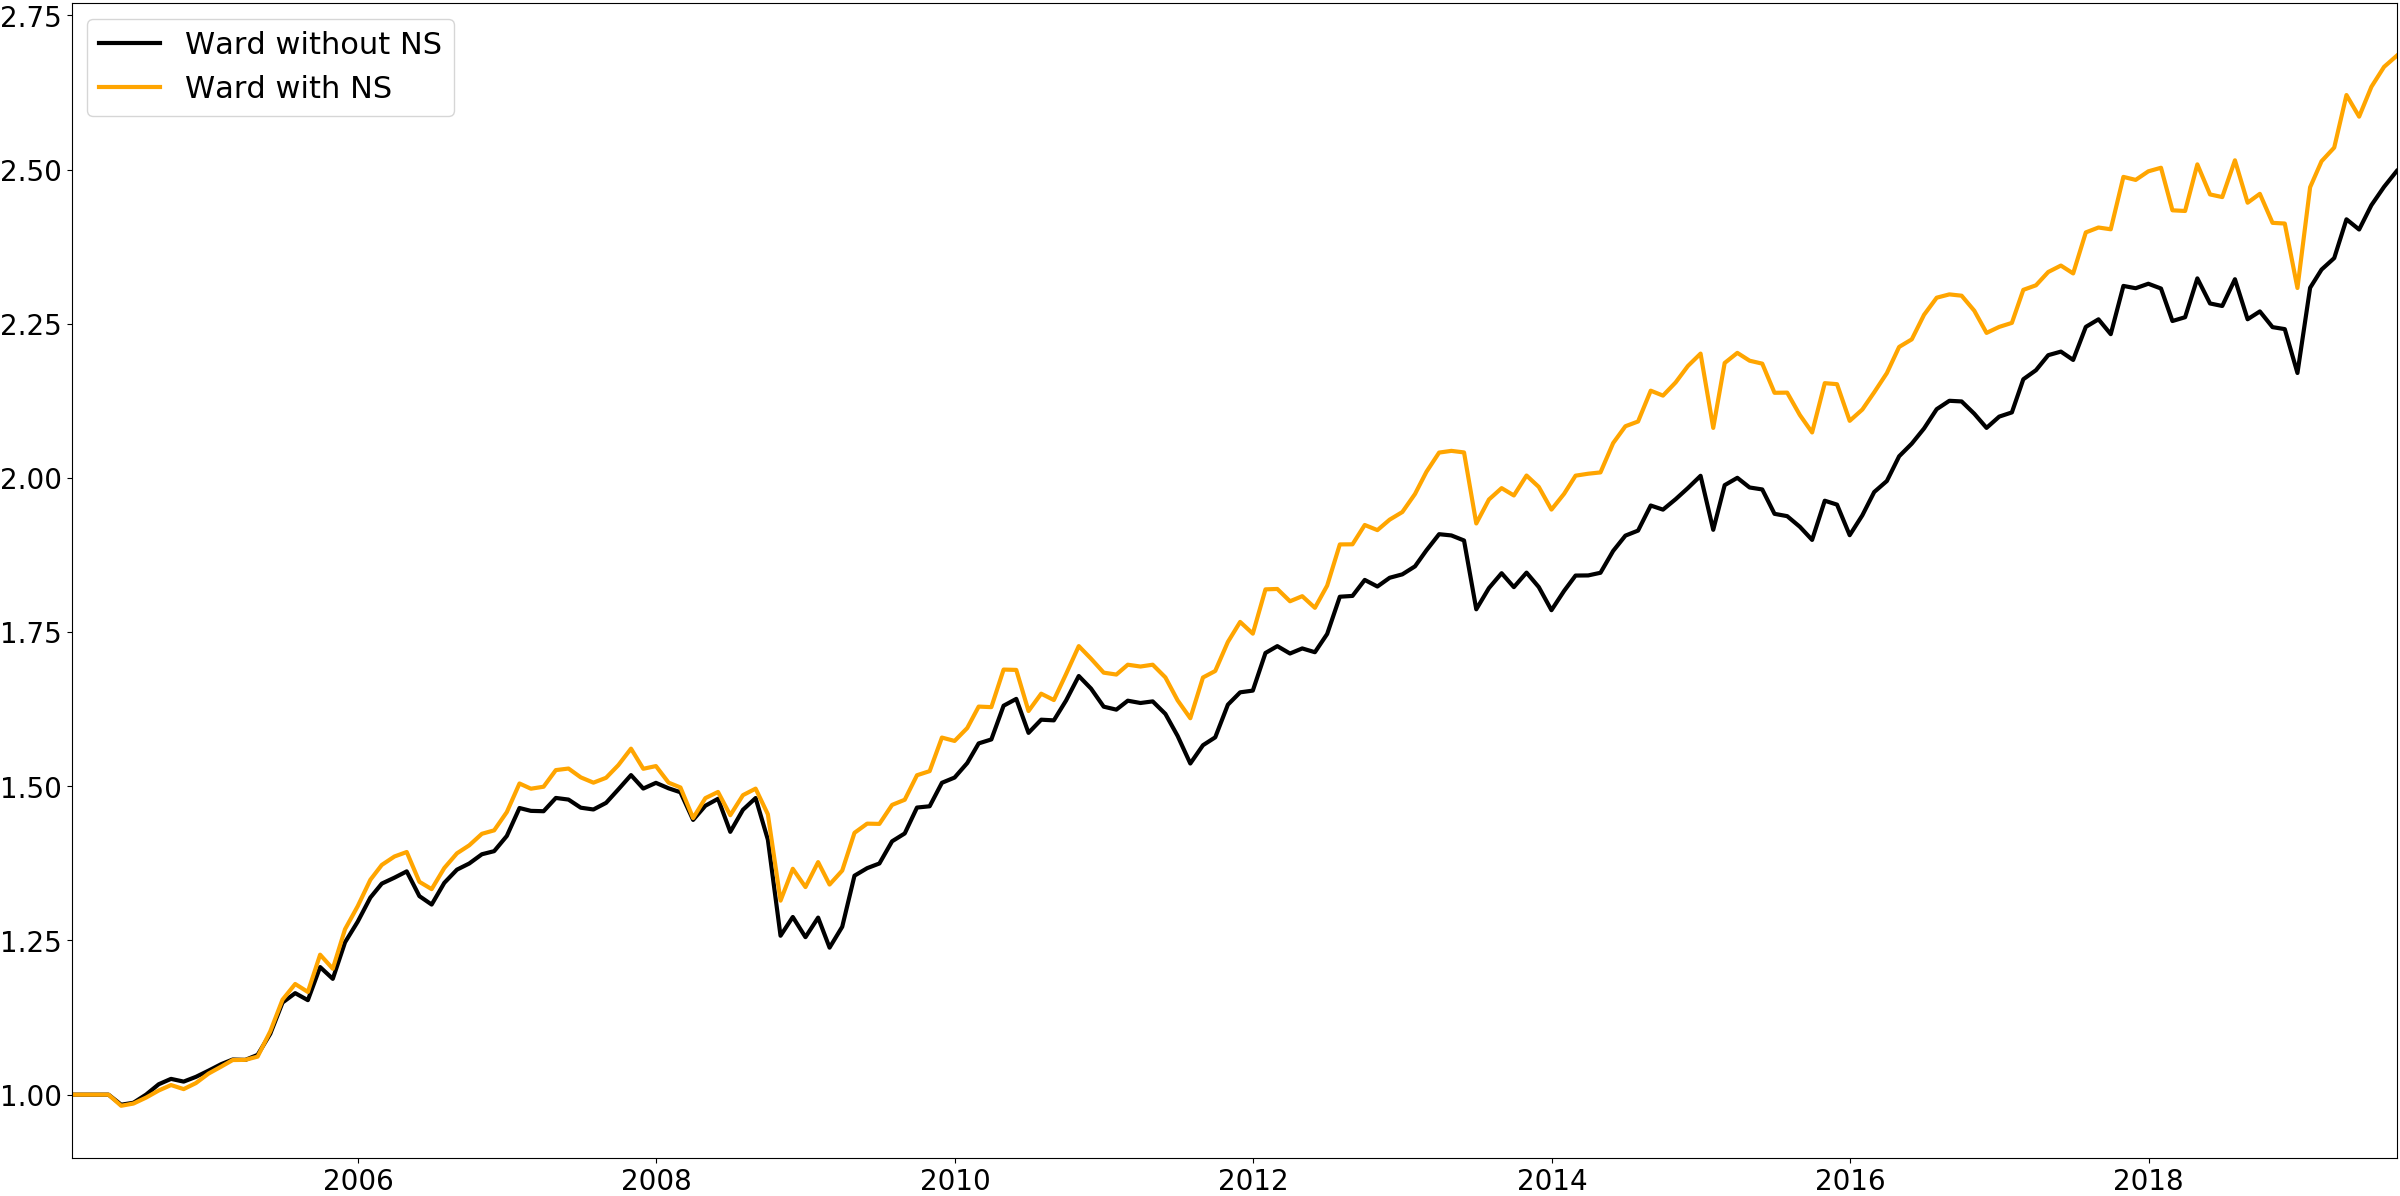
\includegraphics[width=\linewidth]{Plots_and_Tables/perf_noTC_ward_comp_F_2_B_0_LB_12_3_!!}
\caption{Comparison \texttt{ward} clustering approach with and without News Sentiment starting in May 2004.} \label{fig:notc_noNS_perf} % 3 + 2
\end{subfigure}%\hspace*{\fill}

\medskip
\begin{subfigure}{0.8\textwidth}%{0.48\textwidth}
\centering
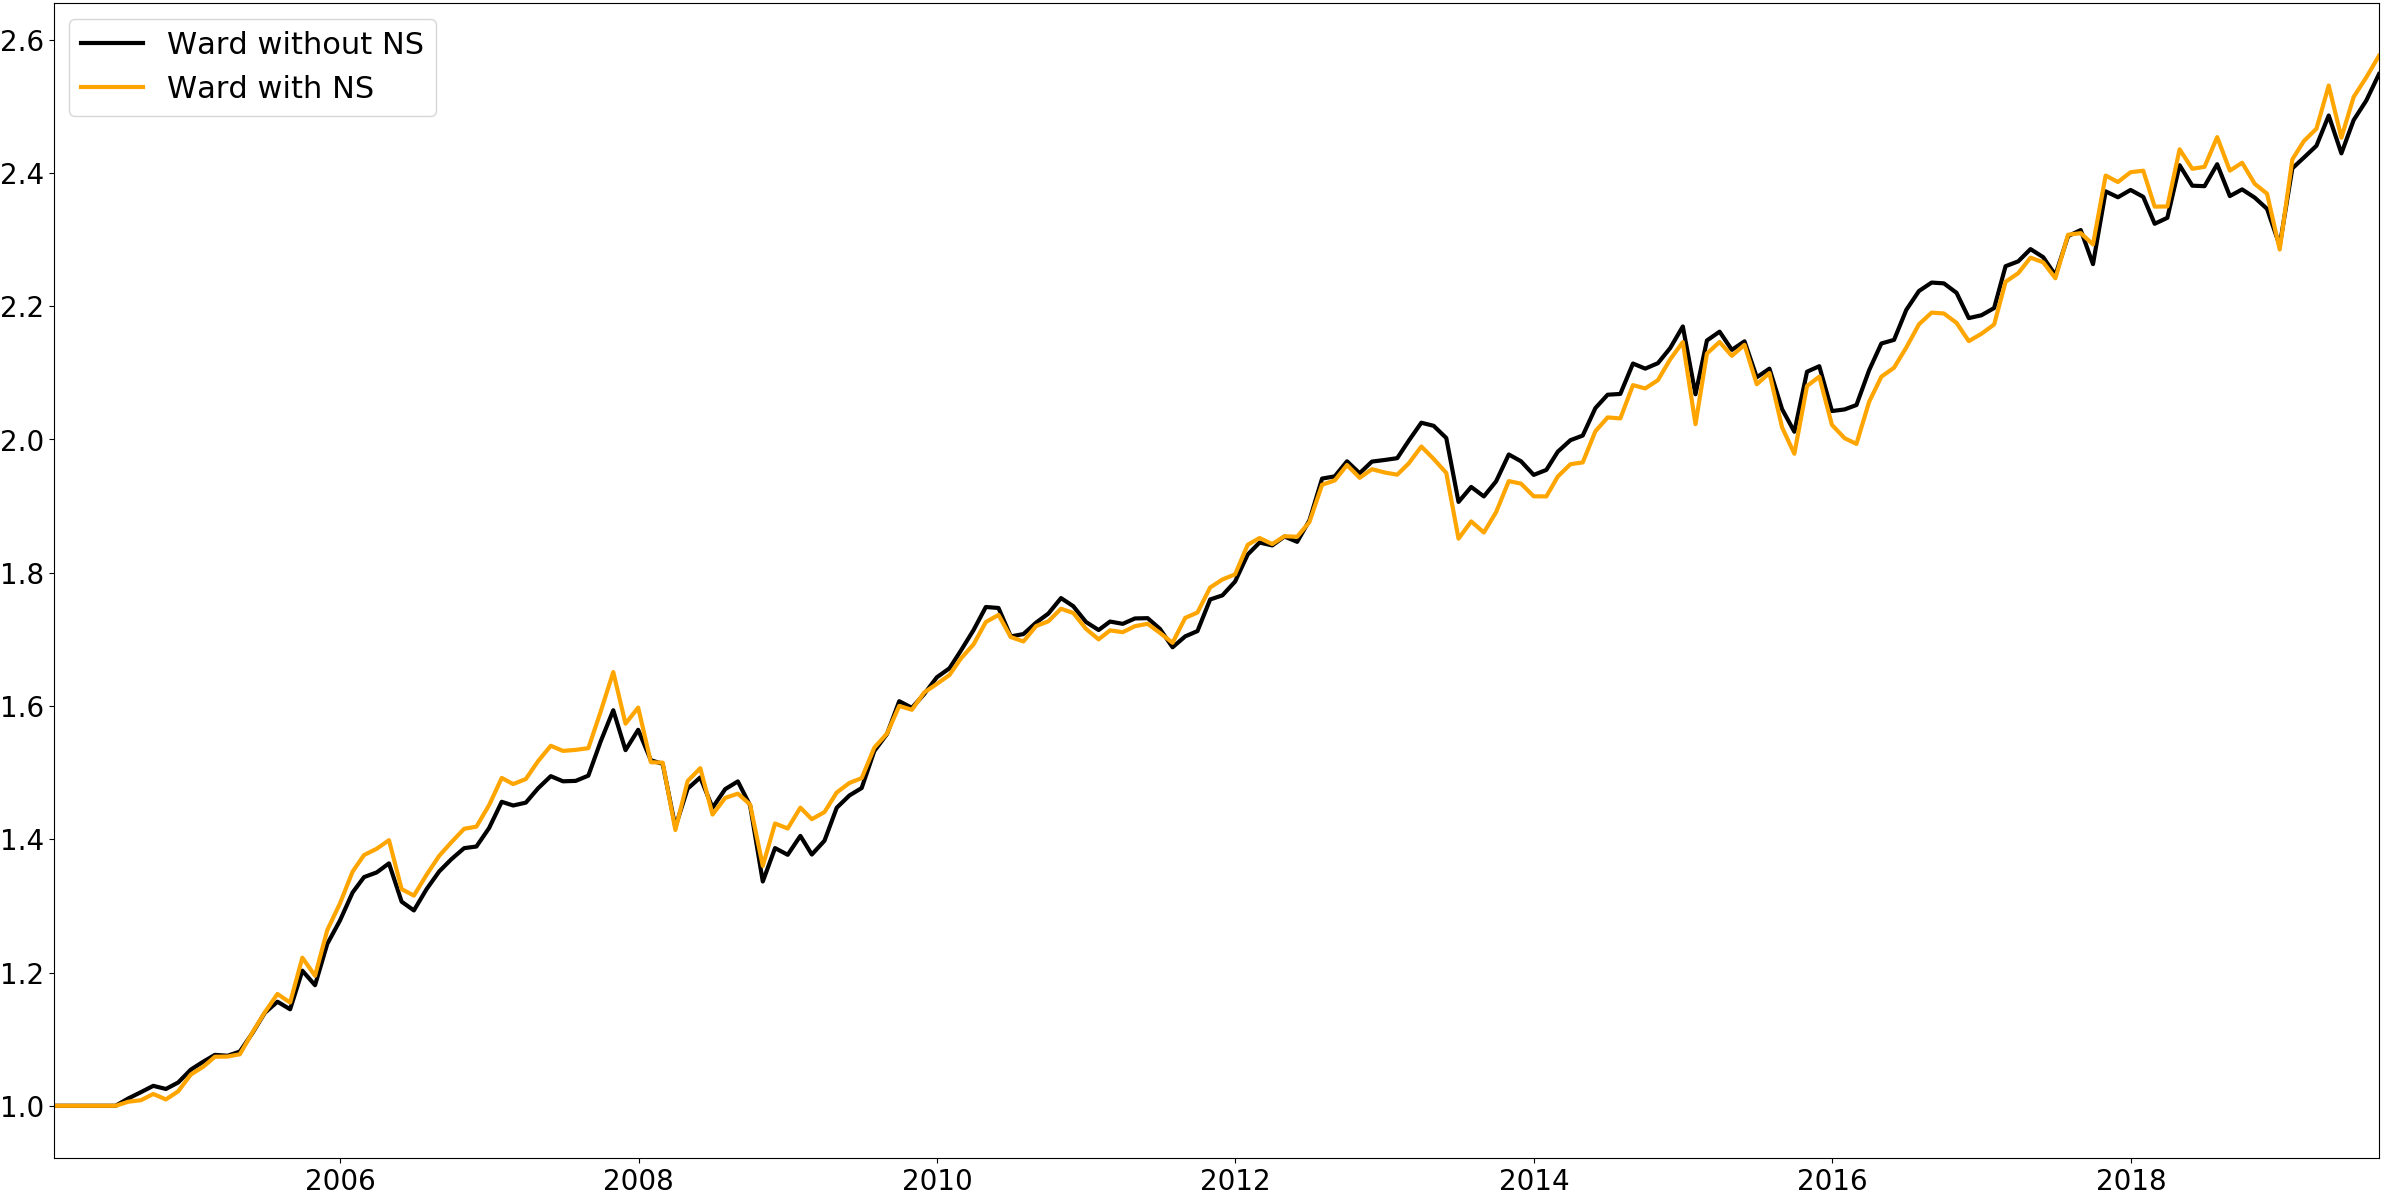
\includegraphics[width=\linewidth]{Plots_and_Tables/perf_noTC_ward_comp_F_2_B_0_LB_12_5_!!}
\caption{Comparison \texttt{ward} clustering approach with and without News Sentiment starting in July 2004.} \label{fig:tc_noNS_perf}
\end{subfigure}%\hspace*{\fill}


\medskip
\begin{subfigure}{0.8\textwidth}%{0.48\textwidth}
\centering
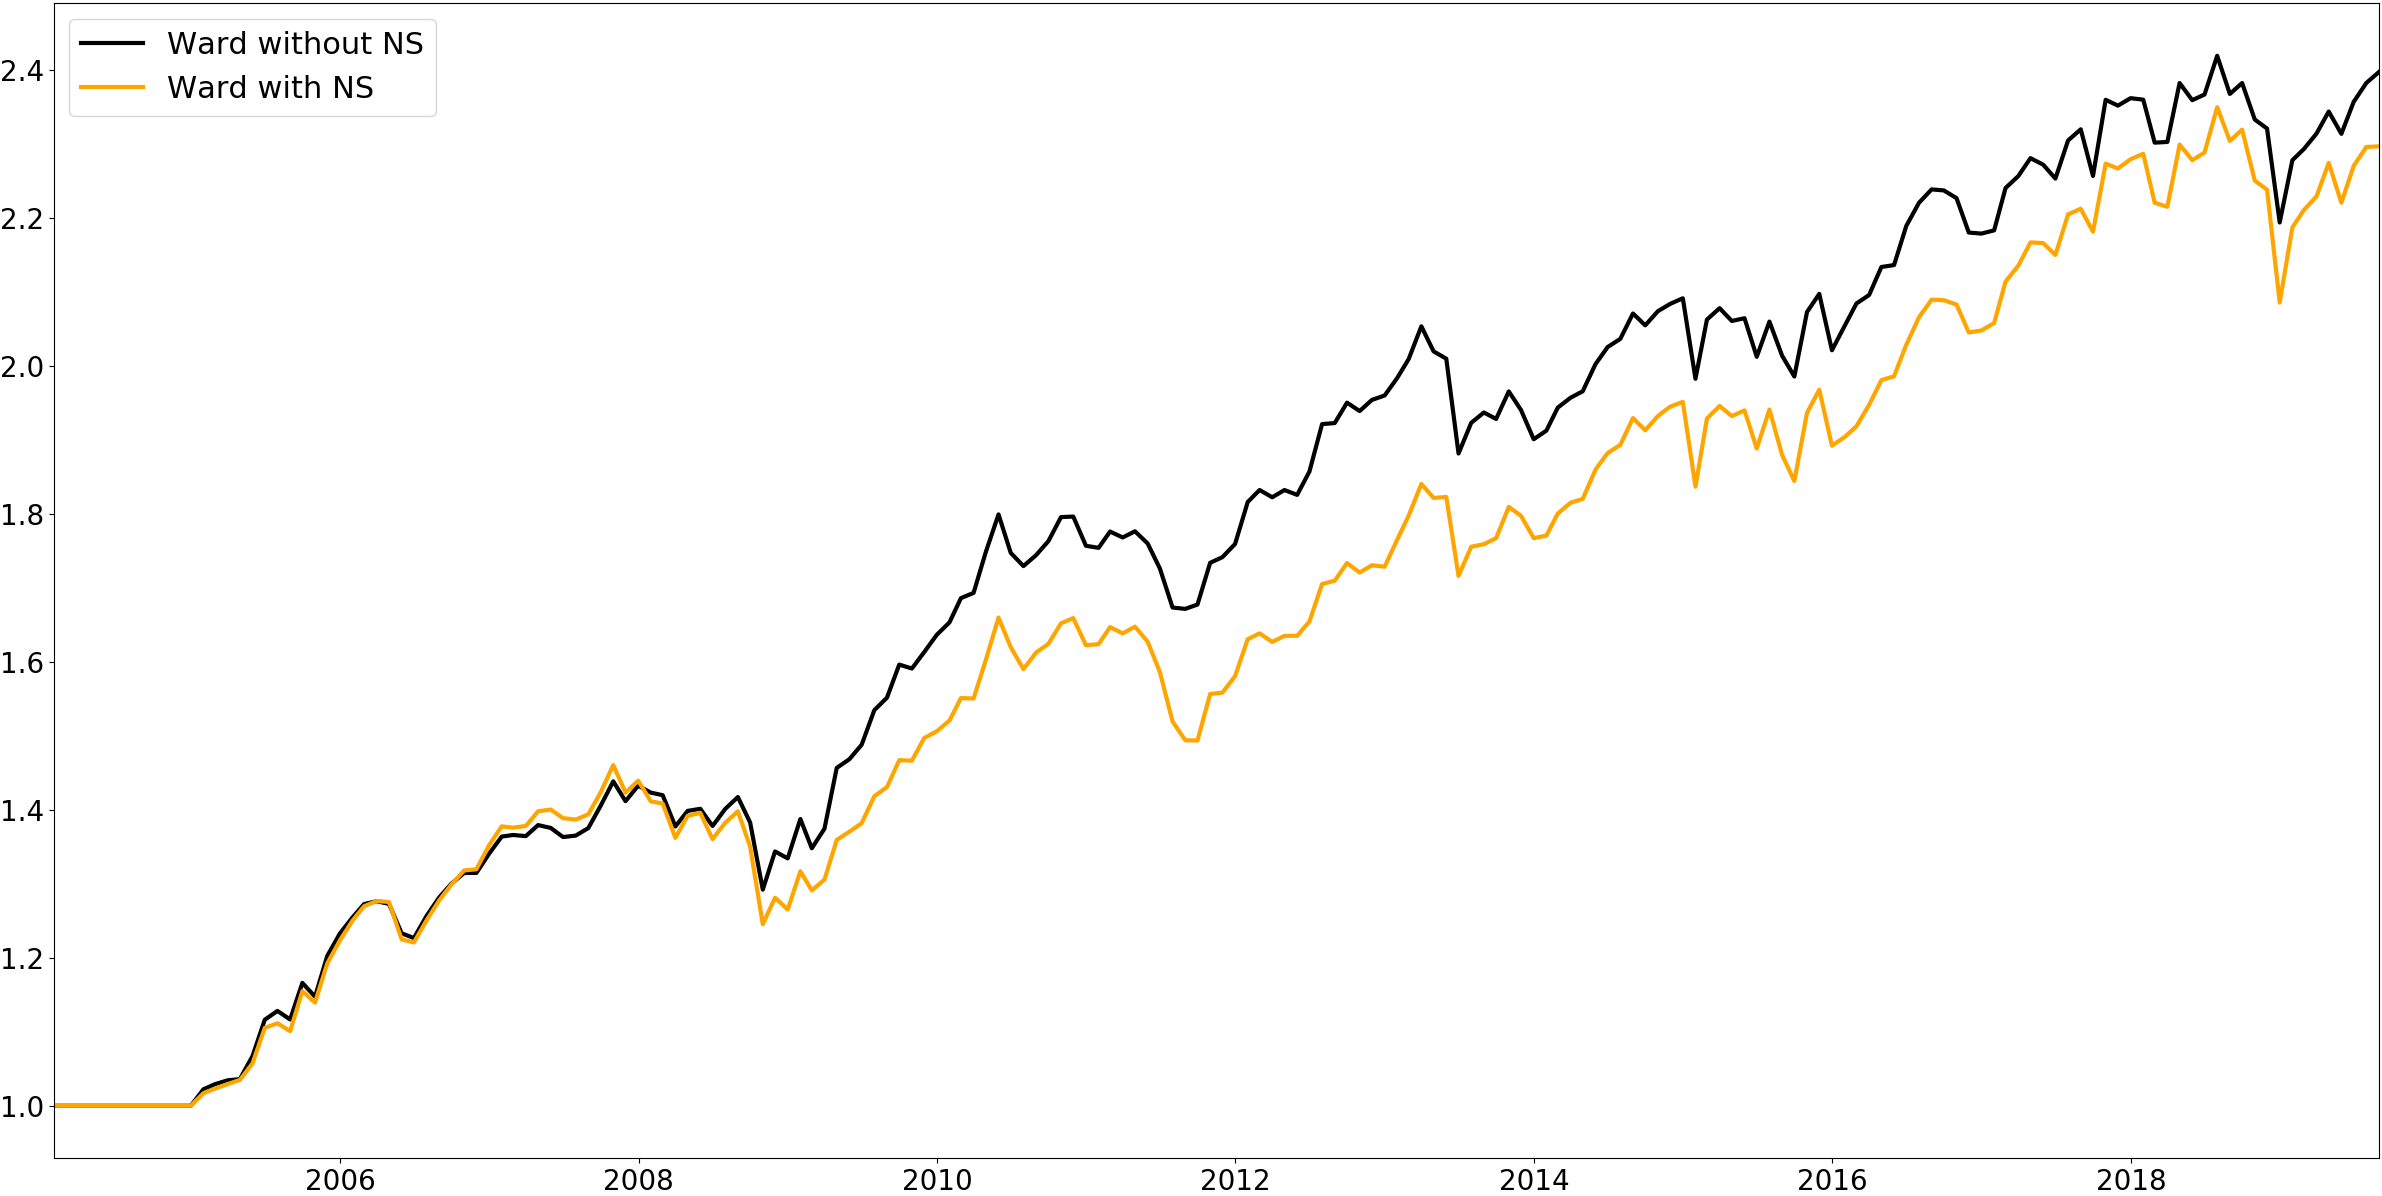
\includegraphics[width=\linewidth]{Plots_and_Tables/perf_noTC_ward_comp_F_2_B_0_LB_12_11_!!}
\caption{Comparison \texttt{ward} clustering approach with and without News Sentiment starting in January 2005.} \label{fig:comp_noNS_perf}
\end{subfigure}%\hspace*{\fill}


\caption{Performance of different strategies without News Sentiment enhancement.} \label{fig:noNS_perf}
\end{figure}
\newpage